\documentclass[10pt]{report}
\setlength{\parindent}{0pt}
\setlength{\parskip}{0,5em}
\usepackage[margin=1in, paperwidth=8.5in, paperheight=11in]{geometry}
\usepackage[utf8]{inputenc}
\usepackage[T1]{fontenc}
\usepackage{polski}
\usepackage[polish]{babel}
\usepackage{lmodern}
\usepackage{multirow}
\usepackage{amsfonts}
\usepackage{graphicx}
\usepackage{placeins}
\usepackage{courier}
\usepackage{listings}
\usepackage{color}
\definecolor{codegreen}{rgb}{0,0.6,0}
\definecolor{codeorange}{rgb}{1,0.54,0}
\lstdefinestyle{CppStyle}{
  belowcaptionskip=1\baselineskip,
  breakatwhitespace=false,
  breaklines=true,
  captionpos=b, 
  frame=below,
  aboveskip=20pt,
  belowskip = 10pt,
  language=C++,
  showstringspaces=false,
  showspaces=false,
  numbersep=5pt,
  numbers=left,  
  numberstyle=\small,
  commentstyle=\color{codegreen},
  keywordstyle=\color{magenta},
  stringstyle=\color{codeorange},
  basicstyle=\small\ttfamily,
}
\lstset{escapechar=@,style=CppStyle}

\title{Projekt na zajęcia e-systemów Java}
\author{
        Sebastian Wilgosz (195963)\\
        Radosław Skiba() }

\makeatletter
\renewcommand{\maketitle}{
\begin{titlepage}
    \begin{center}
        \vspace*{2,5cm} 
        \LARGE\textbf{Edytor map 3D}\par
        \vspace {10mm}
        \large\textbf{\@title}\par
        \vspace{5cm}
    
    	\large\textit{\@author}\par   	  		
    	\vspace {10mm}
    	
    	\large\textit{Termin zajęć:}
    	\large\textit{Czwartek, godz. 17:05}\par
    	\large\textit{Prowadzący:}
       	\large\textbf{dr inż. Tomasz Walkowak}\par
        \vspace{3cm}
        \small \@date
    \end{center}
\end{titlepage}
}
\makeatother
% Pakiety uzywane przez INTRO CHAPTER
\usepackage{framed} 
\newcounter{boxCount}
\stepcounter{boxCount}
\newcommand{\boxy}[2]
{

\begin{framed}
\bf{\arabic{boxCount}. #1 :}
\definecolor{shadecolor}{gray}{.85} % Light Grey
\begin{shaded}
\textnormal{-- #2}
\end{shaded}
\end{framed}
\stepcounter{boxCount}
}

\begin{document}
\maketitle
\tableofcontents
\newpage
\chapter{Cel i zakres projektu}
\section{Zakres projektu}
Niniejszy projekt będzie zawierał opis techniczny i specyfikację kroków, wykorzystania narzędzi niezbędnych do stworzenia aplikacji w środowisku \textbf{Java IEE} .
Projekt będzie uwzględniał następujące etapy : 
\begin{enumerate}
\item{Analiza i Specyfikacja}
\item{Projektowanie}
\item{Implementacja}
\item{Testy}
\item{Ocena i Optymalizacja}
\end{enumerate}

\section{Cel projektu}
Celem projektu jest wykonanie aplikacji serwerowej. 
Aplikacja będzie budowana w oparciu o technologię \textbf{Java IEE}.
Sam sposób wdrożenia programu jak i jego zadania wraz z implementacją będą przebiegały wedle przedstawionego pomysłu, który został wstępnie zaakceptowany przez prowadzącego kurs.
Projekt ma na celu zapoznać Studentów specjalizacji Inżynieria Internetowa z procesem 
budowania oprogramowania obecnie stosowanego w świecie aplikacji serwerowych.
Projekt dodatkowo dzięki wybranemu tematowi pomoże zgłębić technologie strony klienckiej
takie jak \textbf{WebGL} i \textbf{JavaScript}

\chapter{Analiza i Specyfikacja}
\section{Opis słowny zadania}
Celem naszej pracy projektowej jest stworzenie aplikacji zdolnej do tworzenia i zarządzania mapkami 3d terenu.
Niniejsza aplikacja serwerowa ma za zadanie wspomagać tworzenia ciekawych wizualizacji terenu dla osób zajmujących się hobbystycznie jak i zawodowo kartografią.
Tworzone przez użytkowników prace można będzie łączyć, zlecać wykonanie na nich danych obliczeń w celu wykorzystania ich w danym problemie.
Nasz serwis z aplikacją nazwaliśmy \\\textbf{\textit{"Avalanche"}} \textit{[eng. lawina]}, w dalszej części projektowania i założeń podamy bliższe szczegóły naszych kroków projektowych.
Aplikację w przyszłości może uda rozwinąć się do dużo ciekawszych zastosowań.
\section{Specyfikacja wymagań funkcjonalnych}
\boxy{Prezentacja bazy punktów w formie mapy}{Jest to główna funkcja tej aplikacji, ma ona za zadnie z zadanego zbioru danych generować podgląd danego terenu w formie obrotowej mapki w przestrzeni trójwymiarowej.}
\newpage
\boxy{Oddzielne sesje dla każdego użytkownika}{Ponieważ aplikacja będzie zawierała w sobie proces tworzenia jakiegoś elementu terenu niezbędne będzie wyodrębnienie pojedynczych działań na aplikacji w formie sesji użytkowników, którzy swoje gotowe mapki będą mogli dzięki powiązaniu z kontem przechowywać w zdalnej przestrzeni dyskowej} 
\boxy{Wczytywanie mapek z pliku}{Poza wczytywaniem mapek z bazy serwera możliwe będzie wczytywanie wcześniej zapisanych mapek z pliku. Funkcjonalność taka będzie przydatna gdy użytkownik po wykasowaniu maki bądź usunięciu konta, chciałby odtworzyć swoje prace}
\boxy{Łączenie kilku prac w jedną}{Serwer będzie mógł według kilku definiowanych zasad łączyć kilka zasobów w jedną wspólną mapę, taka funkcjonalność będzie przydatna przy tworzeniu pracy opartej na wkładzie kilku użytkowników}
\boxy{Generacja map}{Generacja mapek na podstawie już istniejącej z podanymi zasadami zmiany oraz tworzenie totalnie losowej mapy}
\boxy{Zapisywanie prac na serwerze}{Każda stworzona mapka będzie dostępna niezależnie od miejsca i sprzętu użytkownika poprzez interfejs webowy dostępny w przeglądarce internetowej}
\boxy{Eksport gotowych prac do określonych formatów}{Każdą z gotowych prac będzie można wyeksportować do formatu możliwego do użytku w celu prezentacji/wizualizacji z założenia są to formaty 
\textbf{*.pdf *.jpeg}.}


\section{Specyfikacja wymagań niefunkcjonalnych}
\setcounter{boxCount}{1}
\boxy{Przejrzysty interfejs webowy}{Wymaganiem jest by aplikacja była nie przeładowana dodatkami i prosta w obsłudze dla osób nie posiadających zdolności programistycznych}
\boxy{Szybkość i oszczędność łącza}{Aplikacja powinna większość pracy wykonywać bez potrzeby generowania zbędnego ruchu sieciowego co pomoże zaoszczędzić zasoby klienta}
\boxy{Multiplatformowość}{Aplikacja powinna generować taki sam rezultat niezależnie od platformy sprzętowej klienta}
\boxy{Baza danych MySQL}{Zasób danych powinien być przechowywany na łatwej w obsłudze i bezpłatnej dystrybucji bazy danych, takiej jak np. \textbf{MySQL}}
\boxy{Dane o twórcach jak i projekcie}{Aplikacja będzie zawierała informacje o okolicznościach w jakich powstała i dla jakich celów}
\boxy{Model MVC}{Aplikacja będzie opierać się na modelu MVC}
\boxy{Dokumentacja}{Przebieg procesu powstawania jak i opis funkcjonalności i sposób wykorzystania poszczególnych funkcji będzie zawarty w dokumentacji projektu}
\chapter{Wykorzystywane moduły}
\section{Devise}
Devise to łatwy w użyciu i dostosowaniu do aplikacji moduł rozszerzający Ruby on Rails o proste zarządzanie sesjami. Gwarantuje bezpieczne przechowywanie haseł, kontrolę dostępu, kompletne funkcje logowania, rejestracji, powiadomień mailowych.

\begin{itemize}
\item Napisany jest w rubym
\item Bazuje na silniku RoR, jest całkowicie oparte o strukturę MVC
\item Pozwala na zalogowanie wielu modeli jednocześnie
\item Bazuje na strukturze modułowej - można dołączać tylko te wtyczki, które rzeczywiście potrzebujemy
\end{itemize}

Devise składa się z 10 modułów:

\begin{itemize}
\item Database Authenticatable: koduje i zapisuje zakodowane hasła w bazie danych w celu zapewnienia autoryzacji podczas logowania.
\item Omniauthable: dodaje kompatybilność z mediami społecznościowymi (logowanie przez Facebook, Twitter, Google itp). 
\item Confirmable: wysyła email z potwierdzeniem rejestracji i weryfikuje czy konto jest potwierdzone czy nie.
\item Recoverable: umożliwia resetowanie haseł i wysyła email z instrukcją zresetowania hasła.
\item Registerable: zajmuje się tworzeniem kont użytkowników, także edycji ich profilów i usuwaniem swoich kont. Nie pozwala na edycję innych kont ani na usunięcie nie swojego konta, umożliwia automatyczne zalogowanie po rejestracji
Rememberable: umożliwia zapamiętanie sesji użytkownika w cookies, dzięki czemu pozostaje on zalogowany nawet po zamknięciu przeglądarki.
Trackable: śledzi ilość logowań, adresy IP, rodzaj przeglądarki z której się logowano.
Timeoutable: wylogowuje użytkownika po określonym czasie, jeśli nie stwierdzono żadnej aktywności.
Validatable: dostarcza walidację adresów email oraz haseł. Sprawdza długość hasła, poprawność formatu wprowadzonego adresu email. Jest to opcjonalne i nie przeszkadza w definiowaniu własnych walidacji.
Lockable: blokuje konto po określonej ilości błędnych logowań. Można odblokować konto przez token wysłany na adres email lub po określonym czasie.

\end{itemize}

Devise gwarantuje przechwytywanie przechwytywanie wyjątków, zapewniając bezpieczeństwo oraz generowanie czytelnych komunikatów we wszystkich możliwych przypadkach użycia.


W naszej aplikacji będziemy wykorzystywać następujące moduły devise:

\begin{itemize}
\item database authenticatable
\item registerable
\item recoverable
\item rememberable
\item trackable
\item :validatable
\end{itemize}

\section{ActAsTaggableOn}
ActAsTaggable - to moduł wykorzystywany przez nas do grupowania map oraz użytkowników. Wtyczka ta umożliwia szybkie dodanie funkcji otagowania dowolnego modelu, filtrowanie po tagach, dodawanie wielu tagów jednocześnie czy wyświetlania powiązanej chmury tagów.

Dodatkowe funkcje zapeniane przez ten moduł, to znajdowanie najczęściej i narzadziej używanych tagów, powiązanie wielu rodzajów tagów z jednym modelem (np: tagi jako kategorie, grupy, szkoły - wszystko może być powiązane z modelem użytkownika)

\section{CanCanCan}

CanCanCan to biblioteka do autoryzacji dla Ruby on Rails. Pozwala określić, do jakich zasobów aktualnie zalogowany użytkownik ma dostęp. Wszystkie prawa dostępu są zdefiniowane w pojedynczej lokalizacji (klasie Ability) i nie są powtarzane w kontrolerach, widokach czy zapytaniach do bazy danych.

\section{PG}

Wykorzystywana przez nas baza danych to postgreSQL - wybraliśmy ją, ponieważ serwer Heroku, na którym hostujemy naszą aplikację wykorzystuje tę bazę jako domyślną, co uprościło konfigurację.

Ruby on Rails to framework zaprojektowany do współpracy z bazą danych. Klasa ActiveRecord zawiera zdefiniowany komplet funkcji komunikującej się z bazą, tworzeniem, edycją, czytaniem i usuwaniem rekordów. Jedyne, czego potrzebujemy, by sprawić, by komunikacja z bazą zaczęła działać, to dodanie modułu precyzującego, jaką bazę nasza aplikacja będzie wykorzystywać.

PG - to interfejs dla Ruby umożliwiający współpracę z bazą danych PostgreSql.

\section{Uproszczona składnia}
Aby przyśpieszyć pracę nad aplikacją i ułatwić zarządzanie stylami/skryptami, dzieląc je na wiele plików postanowiliśmy nie wykorzystywać bogatych w niepotrzebne znaki standardowych składni aplikacji webowych. Zainteresowaliśmy się nakładkami na wykorzystywane przez nas języki (HTML, CSS, JavaScript), które po wrzuceniu na serwer produkcyjny są komplikowane i łączone w pojedyncze pliki, by nie generować dziesiątek requestów do serwera.

\begin{itemize}
	\item Slim-Rails - jest to interpreter języka Slim, nakładki na HTML pozwalającej na pominięcie wszystkich tagów zamykających, bazujący na wcięciach (podobnie do składni Python'a).
\item Coffe-Rails - interpreter języka CoffeeScript będącego udoskonaleniem składni JavaScript. Opiera się na tych samych założeniach co Slim czy Sass.
\item Sass-Rails - interpreter języka Sass, będącego nakładką na standardową składnię CSS, usuwający wszelkie nawiasy klamrowe, średniki, umożliwiający definiowanie zagnieżdżonych styli, wprowadzenia zmiennych, czy działań matematycznych.
\item Uglifier - kompressor do assets. Umożliwia minimalizację kompresję plików *.coffee oraz *.sass do zminimalizowanych odpowiedników *.js oraz *.css. Dzięki temu usunięte sa wszystkie białe znaki, a nazwy funkcji zamieniane są na jednoliterowe.
\item Less-Rails - łączy wszystkie pliki assets w jeden, dzieki czemu do serwera idzie jeden request zamiast osobnego requesta na każdy plik ze stylami czy skryptem.
\end{itemize}

\section{TwitterBootstrapRails}
Ta wtyczka umożliwia integrację naszej aplikacji z jednym z najbardziej znanych frameworków frontendowym wyekstraktowanym z Twittera - Bootstrapem.

\section{SimpleForm}
Dodatek umożliwjający łatwe generowanie skomplikowanych formularzy HTML dla dowolnego obiektu.

\section{TurboLinks}
By uniknąć pobierania z serwera skryptób javaScript oraz styli CSS za każdym razem, gdy użytkownik kliknie w link na stronie, używamy turbo linków. Pozwalają one na odświeżenie wyłącznie kodu zawartego między tagami <body></body>, zaś cała sekcja <head></head> jest ładowana tylko raz.

Dzięki temu zabiegowi nasza aplikacja ładuje się wielokrotnie szybciej.

\section{gravastic}
Moduł pozwalający na wyświetlania Gravatarów użytkowników oraz komentujących mapy, bazujac na emailu podanym w formularzu.

\chapter{Modele systemów}
\section{Diagram ERD}

\begin{figure}[ht]

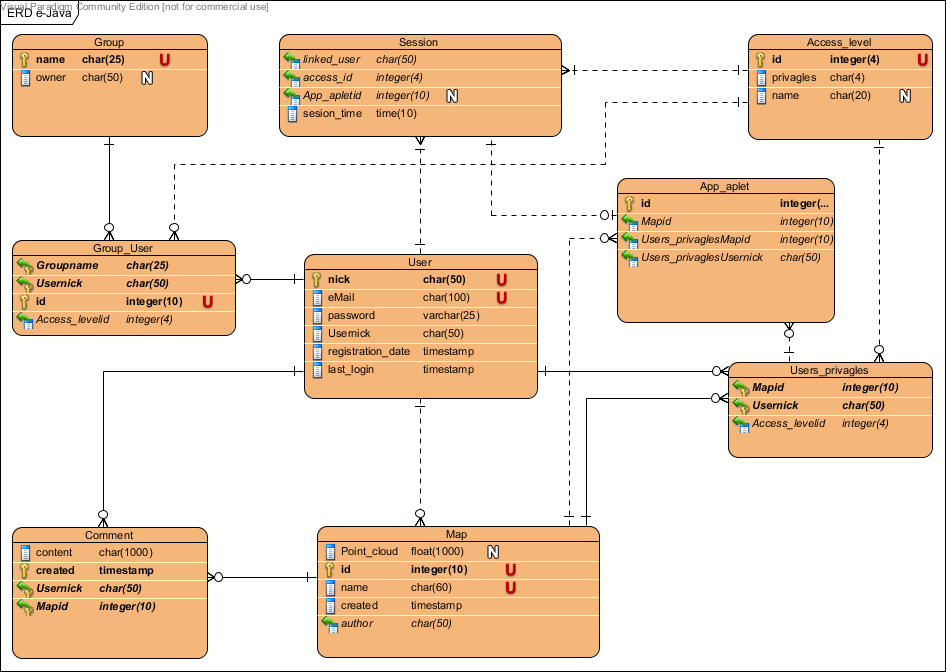
\includegraphics[scale=0.85,angle=270]{img/ERDJava.png}
\caption{Diagram ERD}[b]
\end{figure}
\section{Wizualny diagram modułów}
\begin{center}

\begin{figure}
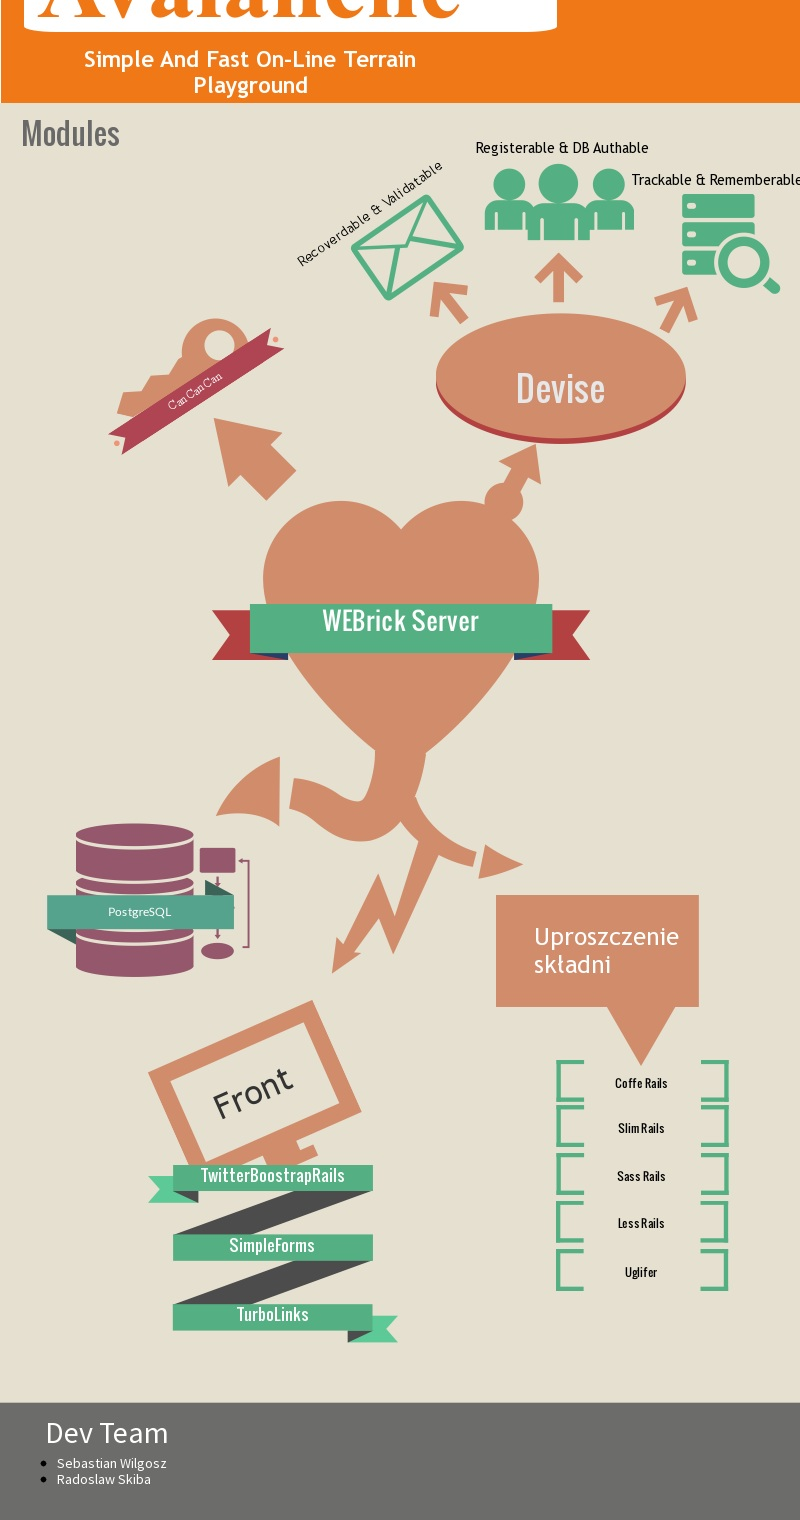
\includegraphics[width=0.90\textwidth,height=0.94\textheight]{img/info.jpg}
\caption{Prezentacja struktury}
\end{figure}

\end{center}
\end{document}
